Dato il grande numero di potenziali fonti per i dati, è necessario ricondurre questi ultimi a una formulazione comune
così da poter sfruttare al meglio le loro potenzialità espressive.
La rappresentazione più basilare consiste nel considerare una traiettoria come l'insieme delle posizioni
spaziali dei punti che la compongono associando a ciascuno l'istante temporale in cui è stato registrato.
Questa formulazione prende il nome di traiettoria grezza (\textit{raw trajectory}), vedi~\cref{fig:chap-1:trajectory}.
Andando a formalizzare quanto detto sopra:

\begin{figure}
  \centering
  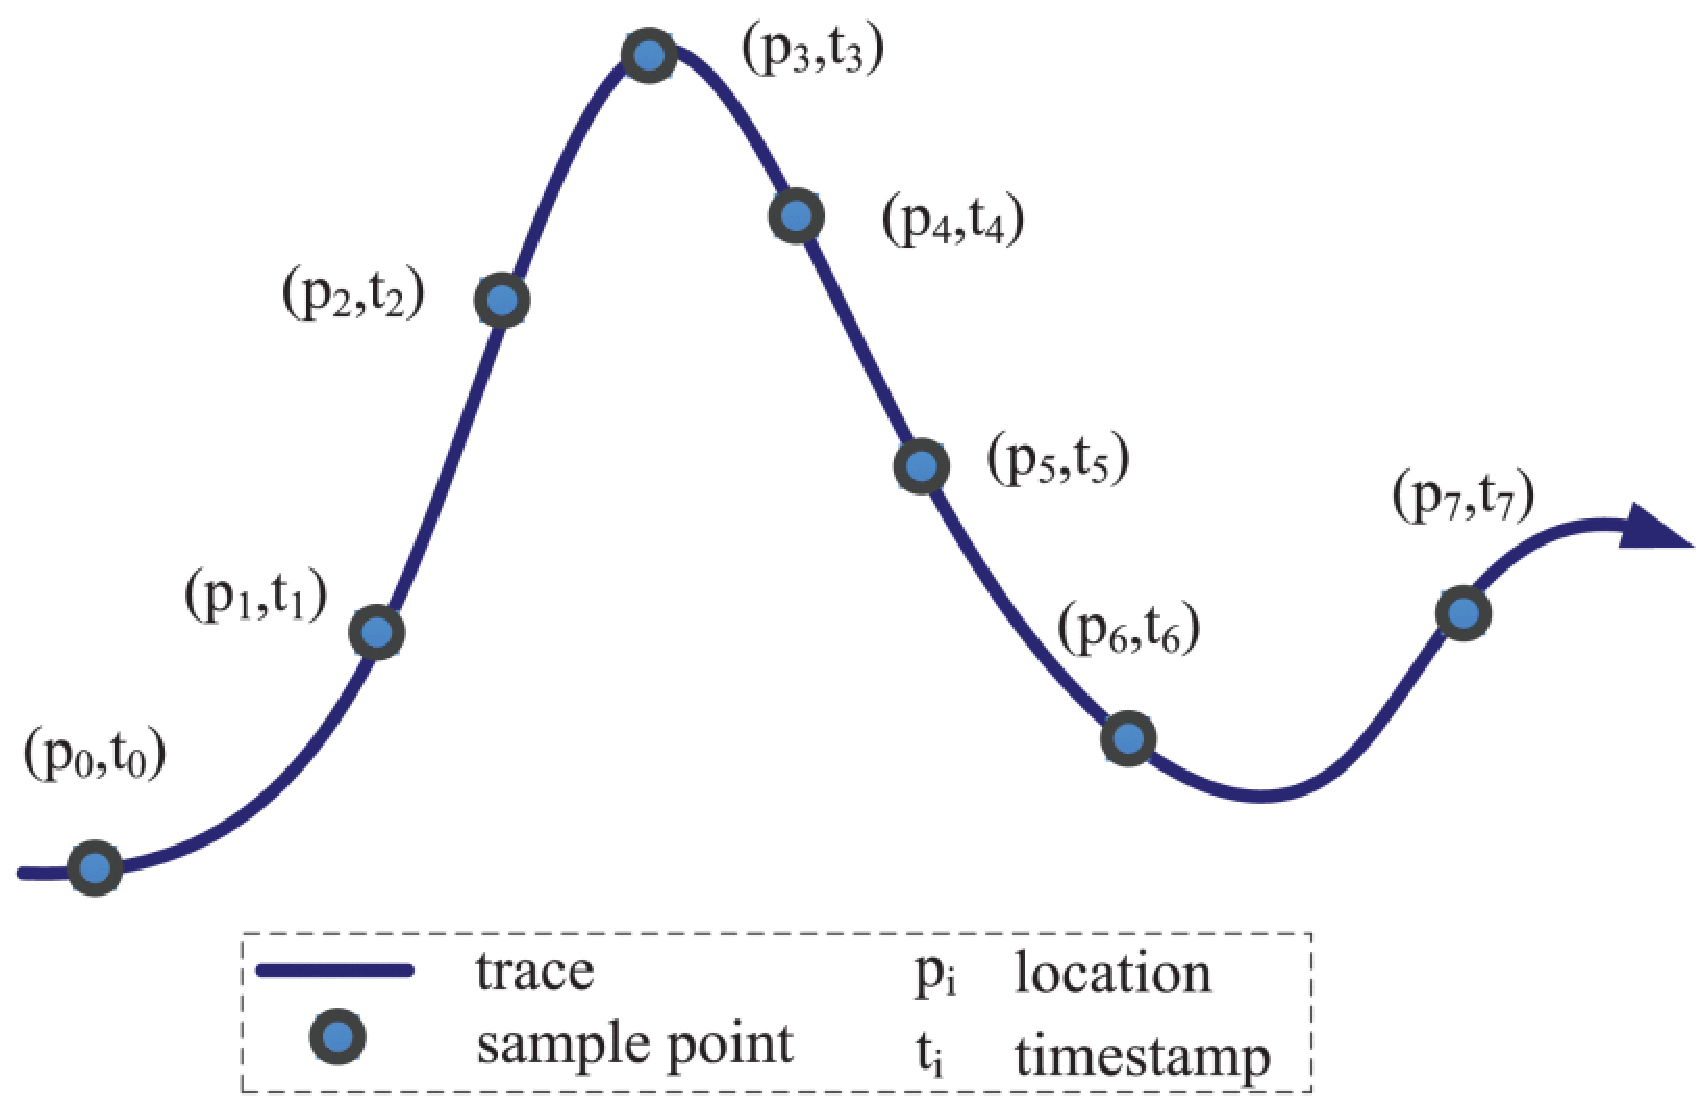
\includegraphics[scale=.7]{/sec-1/trajectory.pdf}
  \caption{Esempio di traiettoria, Fonte:~\cite{Feng2016ASO}}%
  \label{fig:chap-1:trajectory}
\end{figure}

\theoremstyle{definition}
\begin{definition}[Traiettoria]

  Si definisce una traiettoria grezza \(tr\) una sequenza temporale di punti \({p_{t}, p_{t'},\ldots, p_{t''}}\)
  tale che ogni punto \(p_{t}\) è composto da una coppia di coordinate spaziali \((latitude, longitude)\) e un tempo~\(t\).

\end{definition}

Tale formulazione può essere successivamente complicata, ad esempio adottando
una scala unica tra le diverse traiettorie per lo spazio e una per il tempo, oppure aggiungendo ulteriori informazioni, come ad esempio la direzione o altri attributi
dell'oggetto che la genera.

Per aumentare l'espressività della singola traiettoria, può essere utile definire il concetto di sotto-traiettoria, o \textit{subtrajectory}.
Intuitivamente una sotto-traiettoria non è altro che un segmento di una traiettoria relativo a un certo sottoinsieme dello spazio-tempo coperto da quest'ultima.

\begin{definition}[Sotto-traiettoria]

  Date due traiettorie \(tr\textsubscript{i}, tr\textsubscript{j}\) si definisce  \(tr\textsubscript{i}\) sotto-traiettoria di \(tr\textsubscript{j}\) se \(\forall p_{t\textsubscript{i}} \in tr\textsubscript{i}, p_{t\textsubscript{i}} \in tr\textsubscript{j}\).

\end{definition}

A queste definizioni va aggiunto il concetto di sistema di riferimento: si definisce un sistema di riferimento un insieme di
quanti completo e continuo all'interno di una regione spazio-temporale.
I sistemi di riferimento sono fondamentali nel determinare le dimensioni spazio-temporali dei punti delle varie traiettorie,
un esempio su tutti può essere una scala di riferimento espressa in coordinate polari.
Tuttavia è possibile definire anche sistemi di riferimento che utilizzano metriche diverse dalle coordinate sopracitate,
ottenendo così diversi effetti sulla rappresentazione dei dati.
Una traiettoria rappresentata secondo le coordinate di un certo sistema di riferimento si definisce \textit{trajectory abstraction} o astrazione di traiettoria:

\begin{definition}[Astrazione di traiettoria]

  Data una traiettoria grezza \(tr\) e un sistema di quanti spazio-temporali \( ST = \{q_{1},\ldots q_{n}\}\), un'astrazione di traiettoria è definibile come la sequenza di quanti  \( \{q_{i},\ldots q_{j}\}\) ottenuti esprimendo la traiettoria grezza \(tr\) sul sistema \(ST\)  .

\end{definition}

